\section{Design}
\label{sec:design}

The objectives of Section~\ref{sec:threat} require a selected interval to become a value the
operator sets. We derive that from one transaction and defer the hardware realization to
Section~\ref{sec:impl}.

\subsection{A timing model for one transaction}
\label{sec:design:model}

\begin{figure}[t]
  \centering
  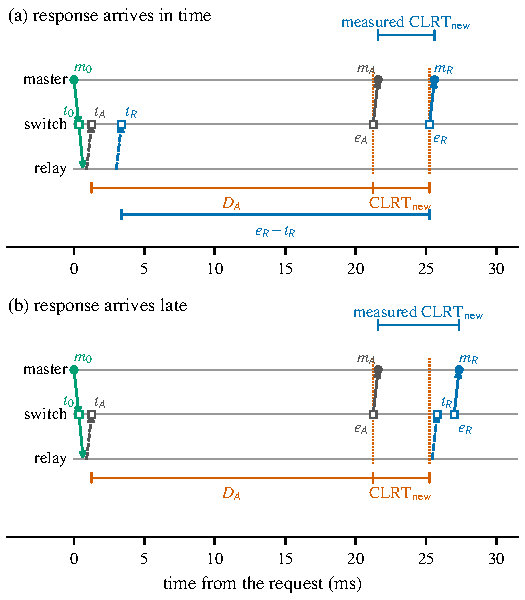
\includegraphics{figures/model/fig_m01_release_timeline}
  \caption{Release timeline of one READ transaction. Time coordinates are illustrative, chosen so
  an arrival and its emission are separable on the page. Both deadlines are computed from the
  acknowledgment's arrival $t_A$: in (a) the response arrives in time and the master observes the
  configured $\mathrm{CLRT}_{\mathrm{new}}$, in (b) it arrives late. The response hold $e_R-t_R$
  is drawn in (a) because the schedule implies it rather than configuring it. Filled circles lie
  on the master-facing link, the only place this work captured anything; open squares are
  switch-side instants that were not captured.}
  \label{fig:timeline}
\end{figure}

Consider one READ transaction, drawn in Figure~\ref{fig:timeline}. The master sends a request.
The outstation answers it twice: first its transport layer acknowledges the request, and later
its application layer returns the response with the data. We write $t_A$ for the instant the
acknowledgment reaches the switch and $t_R$ for the instant the response reaches it. The
switch forwards each packet onward at some later instant, $e_A$ and $e_R$ respectively. The
master therefore observes the interval $e_R - e_A$, up to the propagation and capture delay of
the two packets on the link between them.

That interval carries the information about the device, and on our relay it has a median of
2.116~ms for a poll and a spread of 2.6~ms:
\begin{equation}
\label{eq:clrt-original}
\mathrm{CLRT}_{\mathrm{original}} = t_R - t_A ,
\end{equation}
the time the outstation itself spends between acknowledging the request and producing the answer.
Section~\ref{sec:bg} explains why it identifies the device; here it is the quantity we intend to
remove.

To change what the master sees, the switch holds each packet. We write
\begin{equation}
\label{eq:holds}
D_A = e_A - t_A
\end{equation}
for the \emph{acknowledgment hold}, and we refer to $e_R - t_R$ as the \emph{response hold}
without giving it a symbol of its own, because the schedule below fixes it rather than letting us
choose it. Substituting into the interval the master observes gives the identity that governs the
whole design,
\begin{equation}
\label{eq:clrt-new}
\mathrm{CLRT}_{\mathrm{new}} = e_R - e_A
  = \mathrm{CLRT}_{\mathrm{original}} + (e_R - t_R) - D_A .
\end{equation}

Equation~(\ref{eq:clrt-new}) makes the difference between two kinds of defense concrete. If both
holds are constants, their difference is a constant and the observed interval is the original one
moved by it: the distribution slides along the axis and keeps its width, a spread of 2.6~ms
wherever it is moved to, so an observer who has seen the device before still recognizes it by the
shape. The response hold must instead absorb the variation in
$\mathrm{CLRT}_{\mathrm{original}}$, which we achieve by computing both releases from the same
instant $t_A$. When the acknowledgment arrives, the switch computes both release instants
immediately,
\begin{equation}
\label{eq:schedule}
e_A = t_A + D_A , \qquad e_R = t_A + D_A + \mathrm{CLRT}_{\mathrm{new}} ,
\end{equation}
where $\mathrm{CLRT}_{\mathrm{new}}$ is the interval we want the master to observe. These are the
\emph{scheduled} release instants. A packet's realized departure follows its scheduled instant by
the time the blocker queue takes to drain and by the queue's own service, which
Section~\ref{sec:impl} describes and Section~\ref{sec:eval:limits} measures on an instrumented
build, so the equalities here describe the schedule rather than the wire. We call this
value the \emph{configured} $\mathrm{CLRT}_{\mathrm{new}}$, and we call what the master actually
records the \emph{measured} $\mathrm{CLRT}_{\mathrm{new}}$; Section~\ref{sec:eval} reports how far
apart the two are. Because both release instants derive from $t_A$ and neither from $t_R$, the term
$\mathrm{CLRT}_{\mathrm{original}}$ cancels in~(\ref{eq:clrt-new}) and the observed interval is
the configured one. The response hold is therefore implied rather than chosen,
\begin{equation}
\label{eq:coupling}
e_R - t_R = D_A + \mathrm{CLRT}_{\mathrm{new}} - \mathrm{CLRT}_{\mathrm{original}} .
\end{equation}
Equation~(\ref{eq:coupling}) is why the three quantities cannot be picked independently: once the
acknowledgment hold and the configured $\mathrm{CLRT}_{\mathrm{new}}$ are fixed, the response hold
follows from whatever the device did on that transaction, and so varies from one transaction to
the next exactly as much as the device does.

This holds only while the response exists in time to be released on schedule. The switch can
delay a packet but cannot emit one it has not received, so~(\ref{eq:schedule}) requires
\begin{equation}
\label{eq:availability}
t_R \le t_A + D_A + \mathrm{CLRT}_{\mathrm{new}} .
\end{equation}
The acknowledgment may leave before the response arrives; that ordering is normal and does not by
itself imply a lost packet. When~(\ref{eq:availability}) fails the deadline is already past when
the response appears, so the switch marks it late and commits it to the response-hold queue, from
which it leaves when that queue next serves it, and the master observes an interval larger than
the configured value, as in Figure~\ref{fig:timeline}(b). One read-lane exchange in a thousand
answers too late to be scheduled. We report those rather than excluding them, because they are the
boundary of the mechanism and not a defect of the measurement.

The holds decide what the master observes \emph{between} the two packets, not how long it waits
for the answer itself, which is the quantity an operational requirement constrains. Write $D_R$
for that: the response's whole journey from the outstation transmitting it to the master receiving
it. We do not measure $D_R$, nor the portion of it from the switch onward, because only the
master-facing link is instrumented: $m_R$ is captured while $t_R$, the response's arrival at the
switch, is not. The quantity
\begin{equation}
\label{eq:resplatency}
m_R - t_R \le D_R
\end{equation}
is therefore a modelled partial journey, written from the model's endpoints rather than from
timestamps we hold, and full $D_R$ remains unmeasured.

Two terms make up the observed portion, $(e_R - t_R) + (m_R - e_R)$: the time the switch holds the
response and the path from the switch to the master. The hold itself divides once more, into the
wait to the release deadline, the interval $\varepsilon$ from that deadline to the end of
blocking, because the switch stops blocking a queued packet only once the queue gating it has
drained, and the service that follows. Those three sum to the hold rather than adding to it.
Consequently neither the response hold nor the configured $\mathrm{CLRT}_{\mathrm{new}}$ is the
response latency, and the three are not separately selectable: fixing $D_A$ and the configured
interval fixes the hold, which in turn consumes part of whatever the application deadline allows.
Section~\ref{sec:eval:limits} reports what we measured of $\varepsilon$ and on which build.

\subsection{Choosing the holds and the configured interval}
\label{sec:design:params}

The model leaves three quantities to decide: the acknowledgment hold $D_A$, the configured
$\mathrm{CLRT}_{\mathrm{new}}$, and, through~(\ref{eq:coupling}), the response hold that
follows from them. Each is limited by a different constraint.

The acknowledgment hold is limited in principle by the transport. Holding an acknowledgment delays the feedback the master's TCP uses to decide that a segment
is lost. Consequently, a hold approaching the master's retransmission timeout would make the
master resend a request the outstation had already answered.

That timeout has to be measured, not assumed.
RFC~6298~\cite{paxsonComputingTCPsRetransmission2011} recommends rounding it up to a second, but
that is a recommendation about a minimum and not a property every stack exhibits: on our master an
unacknowledged request is repeated after 201~ms. The 20~ms hold we evaluate consumes about a tenth
of that, and a hold of a few hundred milliseconds would begin to race it. We do not argue that the
timer's adaptivity makes a constant hold safe, because adaptation says nothing about the first
delayed exchange, a reconnection where the timer restarts, or a policy change mid-session.

In practice the transport bound is not the one that binds. The mechanism sustains a hold with a
budget on blocker passes rather than a wall clock, and from that budget, an assumed service rate,
a conservative bound on the outstation's acknowledgment latency, measured detection and release
terms and a safety margin, the control plane computes a horizon $H$ of 30.8~ms and an admissible
budget of 24.8~ms. Three limits act here and we keep them apart: the horizon is advisory and is
what the admission arithmetic reports; a separate clamp refuses any acknowledgment hold above
40~ms outright; and the sweep of Section~\ref{sec:eval:policy} deliberately installs settings past
the horizon to find where the mechanism leaves its operating region. None is a deadline the data
plane enforces, and the distinction matters because a pass budget bounds how many passes are
\emph{serviced}: under strict priority a lower-priority reservoir can be starved while a
higher-priority one is still being served, so one budget does not translate into one elapsed time
for every queue. The sweep of Section~\ref{sec:eval:policy} shows the consequence directly:
at a configured acknowledgment hold of 36~ms the median request-to-acknowledgment interval
saturates at 31.07~ms, well short of the configured value, while the median request-to-response
interval for the same point is 40.58~ms and the median CLRT is 9.51~ms rather than the
configured 4~ms. The acknowledgment reaches a ceiling; the response does not stop at it. That
saturation is an observed transition for the acknowledgment lane at this configuration, not a
release deadline the hardware guarantees for every held packet.

The configured $\mathrm{CLRT}_{\mathrm{new}}$ is limited by the operation, and through $D_R$
rather than directly: what an operator can accept is a bound on how long the answer takes to
arrive, not on the gap between the two packets that carry it. We could not verify a communications
requirement that fixes such a bound for a DNP3 poll or a select-before-operate control on a
distribution relay. The only numeric deadline we could verify from primary documentation is the
relay's own select-to-operate timeout, documented default
1.0~s~\cite{selSEL751AInstructionManual}, which governs how long a select stays armed rather than
how quickly a response must return, and timing classes defined for other protocols do not transfer
to a DNP3 poll merely because their numbers are convenient.

We therefore treat the setting as a deployment choice rather than a compliance question, state the
value we tested, 4~ms, and report the response latency the mechanism produces, about 23~ms more
than the device alone, so an operator with a requirement of their own can check it against those
numbers.

Together the two set what the mechanism costs. Their sum
\begin{equation}
\label{eq:budget}
D = D_A + \mathrm{CLRT}_{\mathrm{new}}
\end{equation}
is the release budget: by~(\ref{eq:availability}) it decides which transactions the switch can
place on the schedule at all. A larger budget covers more of the device's own response-time
distribution and costs more delay on every transaction it covers: at $D=24$~ms it covers 99.9\% of
them for about 23~ms of added latency. $D$ is the budget and not the delay added to each exchange,
since a transaction the outstation answers quickly is held longer than one it answers slowly, so
the added delay is at most $D$ rather than equal to it.

Because the budget and the observable are different quantities, an operator can fix the cost and
still choose the feature: holding $D$ at 24~ms, we installed configured values from 1~ms to 22~ms
and the master observed each one while the added delay stayed the same.
Section~\ref{sec:eval:policy} reports that sweep and the point at which the realized hold stops
tracking the requested one.

The model says nothing about what $\mathrm{CLRT}_{\mathrm{new}}$ should be, so the framework and
the policy it carries are separate. We chose a constant, because it removes the device's variation
entirely and is the simplest policy to state and to check. A schedule could instead draw the value
from a distribution or make it a function of the operation, and the same mechanism would carry it;
we implement and evaluate only the constant setting.

\subsection{The control transaction is timed from the request}
\label{sec:design:control}

A select-before-operate control command differs in one way that matters here: the framework holds
the command itself before it reaches the relay, separating the moment the master issued the
command from the moment the relay acts on it. The outstation's acknowledgment cannot be the
reference instant, because it does not exist until after the command has been released, and any
deadline measured from it would carry the length of the command hold into the interval the master
observes. We therefore time the control lane from the request. When
the OPERATE arrives at $T_0$, the switch releases it toward the relay after an internal
delay $J$. It places the acknowledgment and the solicited response the master sees at configured
offsets from $T_0$,
\begin{equation}
\label{eq:control}
e_{\mathrm{ack}} = T_0 + A , \qquad e_{\mathrm{or}} = T_0 + R .
\end{equation}
Consequently, the interval the master observes is
\begin{equation}
\label{eq:optime}
O = e_{\mathrm{or}} - e_{\mathrm{ack}} = R - A ,
\end{equation}
in which $J$ does not appear, so the relay-facing release time can vary while the master-facing
interval does not, and an observer cannot subtract a known offset to recover it.

The control plane checks that $A$ exceeds the largest admissible $J$ plus the outstation's own
acknowledgment latency before it installs the values, since a deadline the switch cannot honor
would fail open rather than protect. In our experiments $D_A$ is 20~ms, $\mathrm{CLRT}_{\mathrm{new}}$ is 4~ms, and $R - A$ is
also 4~ms, so the two lanes present the same value to the observer.

\subsection{What the design does not change}
\label{sec:design:boundary}

The mechanism replaces one interval per lane and leaves the rest of the exchange as it was. The
DNP3 function codes remain in plaintext and every packet's direction remains visible, so an
observer can still tell a poll from a control command by reading the packet, and the
request-to-acknowledgment interval still contains the outstation's own acknowledgment latency,
displaced by the constant $D_A$ but not reshaped by it. The switch forwards the packets it
received without padding them, injecting new ones or editing any DNP3 field, which is what the
plaintext setting requires and which leaves every size feature as it was. It does change when
packets leave, so it is not a claim about arrival order.
Section~\ref{sec:eval:ro3} reports what an attacker allowed to retrain on the obfuscated traffic
still recovers from the features that remain.
